% ABOUTME: Dataset quality, sensor selection and RUL target rationale for FD001.
% ABOUTME: Training decisions and final descriptive test evidence produced by notebooks/01_eda.ipynb (issue #3).
\section{Dataset and Exploratory Analysis}
\label{sec:data}

\subsection{Dataset and quality checks}
We use the FD001 subset of NASA C-MAPSS, a simulated turbofan degradation
benchmark with one nominal operating condition and one fault mode: high-pressure
compressor degradation~\cite{saxena2008damage}. Each observation contains an
engine identifier, a cycle number, three operating settings and 21 sensor readings.
The training set contains 20,631 observations from 100 engines run to failure.
All sensor and target decisions use this training set. A final subsection adds
descriptive test plots approved in review; no earlier choice was revisited.

We found no missing cells, duplicate rows or duplicate engine-cycle keys.
Cycles start at one and are consecutive within each engine, so no imputation
or row removal was needed. Recorded lifetimes range from 128 to 362 cycles,
with median 199 and mean 206.31 cycles. Figure~\ref{fig:eda-lifetimes} shows
the distribution of lifetimes, counting each engine once, and the RUL
distribution, counting every cycle. The latter weights longer histories more
heavily. These descriptive distributions are not model evaluation results.

\begin{figure*}[t]
  \centering
  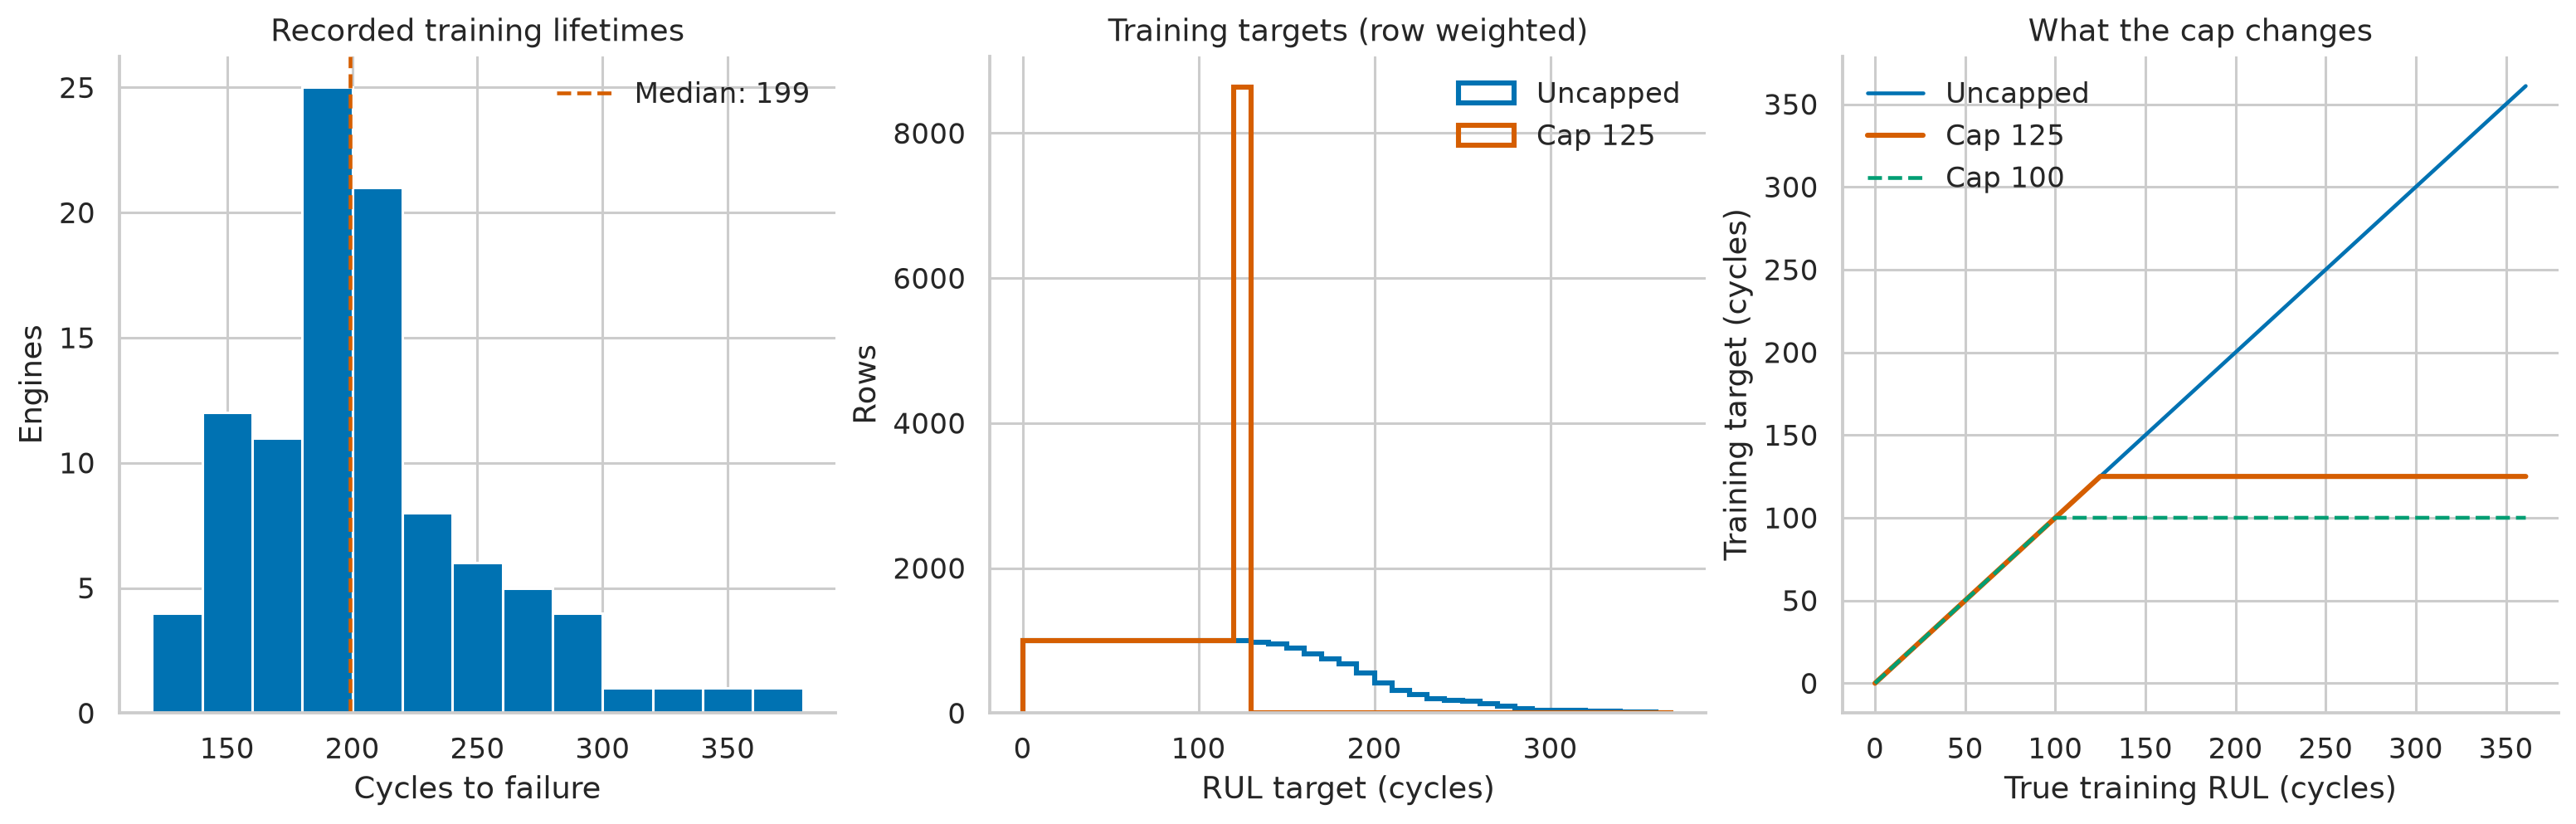
\includegraphics[width=\textwidth]{../figures/eda_lifetimes_rul.png}
  \caption{Training lifetimes, uncapped and capped training targets, and the
  effect of caps of 100 and 125 cycles. The cap changes labels, not the number
  of observations.}
  \label{fig:eda-lifetimes}
\end{figure*}

\subsection{Operating settings and sensor selection}
Settings 1 and 2 vary slightly around zero, while setting 3 is exactly 100.
The scatter plots in Fig.~\ref{fig:eda-settings} are consistent with the
single nominal operating condition specified by NASA. A noisy cloud alone
does not establish a physical regime count; no regime clustering is fit here.

\begin{figure}[t]
  \centering
  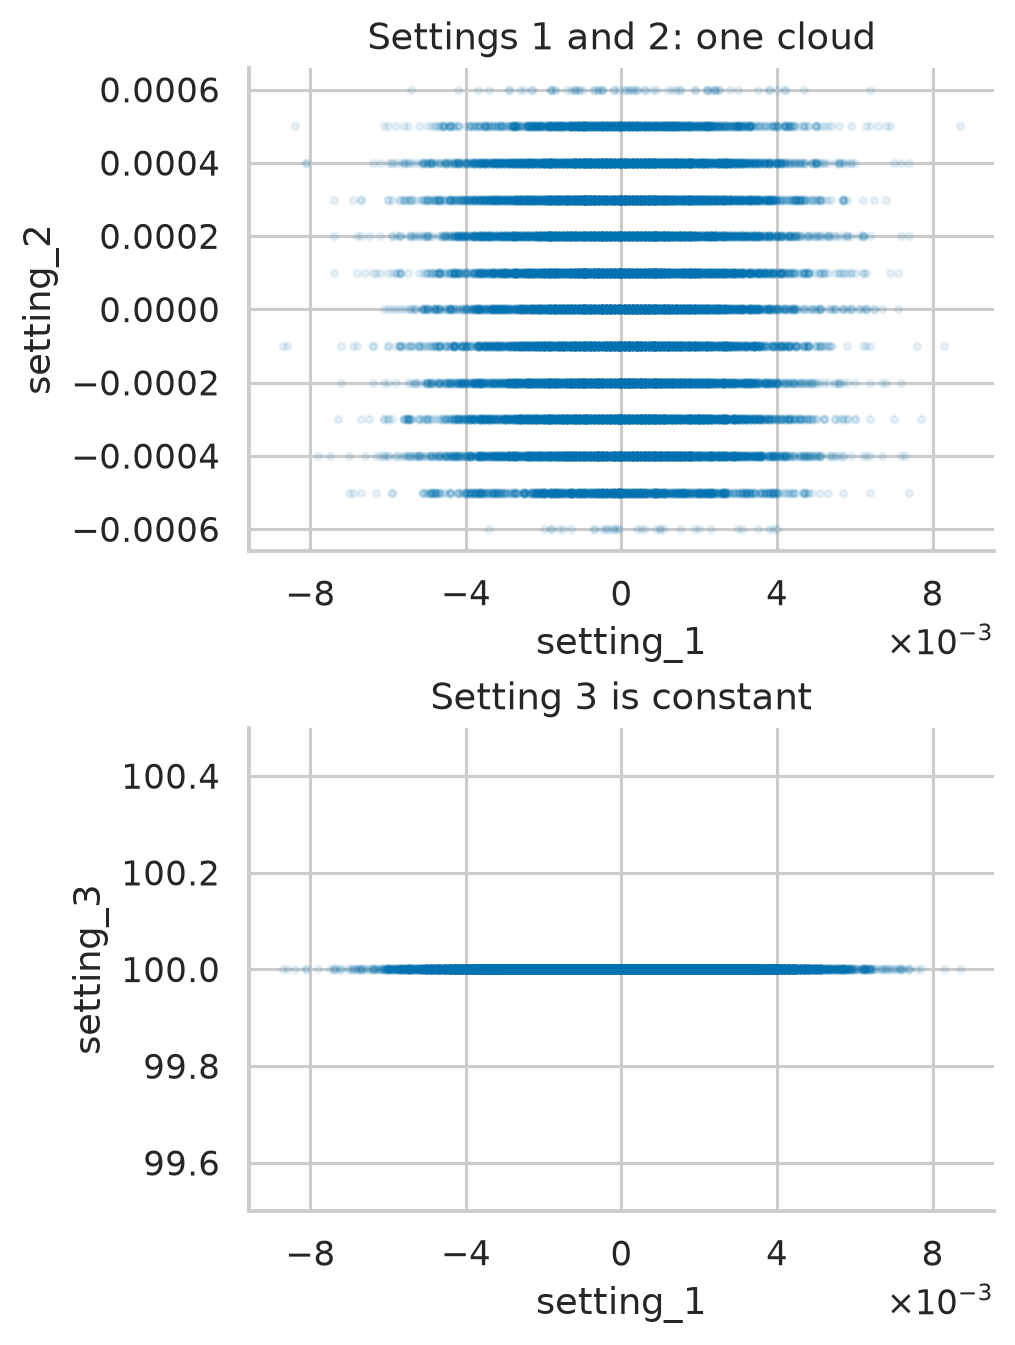
\includegraphics[width=\columnwidth]{../figures/eda_operating_settings.png}
  \caption{Training operating settings: a cloud around zero for settings 1
  and 2, and a constant value for setting 3.}
  \label{fig:eda-settings}
\end{figure}

We compute sample standard deviation, range, distinct-value count and
dominant-value fraction for each sensor. Raw standard deviations are in
different physical units, so an absolute variance threshold would not give
a fair comparison. Sensors $s_1,s_5,s_{10},s_{16},s_{18},s_{19}$ each have
one unique reading and are removed as exact constants. Tiny nonzero
standard deviations for some constants are floating-point roundoff.

We also remove $s_6$, whose only recorded levels are 21.60 and 21.61,
consistent with quantization or rounding at the recorded precision. Its standard
deviation is approximately 0.001389: 20,225 readings are 21.61 and 406 are 21.60.
The 98.03\% dominant share is descriptive, not a selection threshold.
This FD001 choice matches the 14-sensor set listed by Liu et al.~\cite{liu2021rul},
Section 4.2; it does not prove zero predictive information.
The resulting 14 retained sensors are
$s_2,s_3,s_4,s_7,s_8,s_9,s_{11},s_{12},s_{13},s_{14},s_{15},s_{17},s_{20},s_{21}$.
Sensor $s_{17}$ is quantized but has 13 distinct readings and is retained.
Figure~\ref{fig:eda-sensors} summarizes this evidence; the same list is
exported as \texttt{USEFUL\_SENSORS} for feature engineering.

\begin{figure}[t]
  \centering
  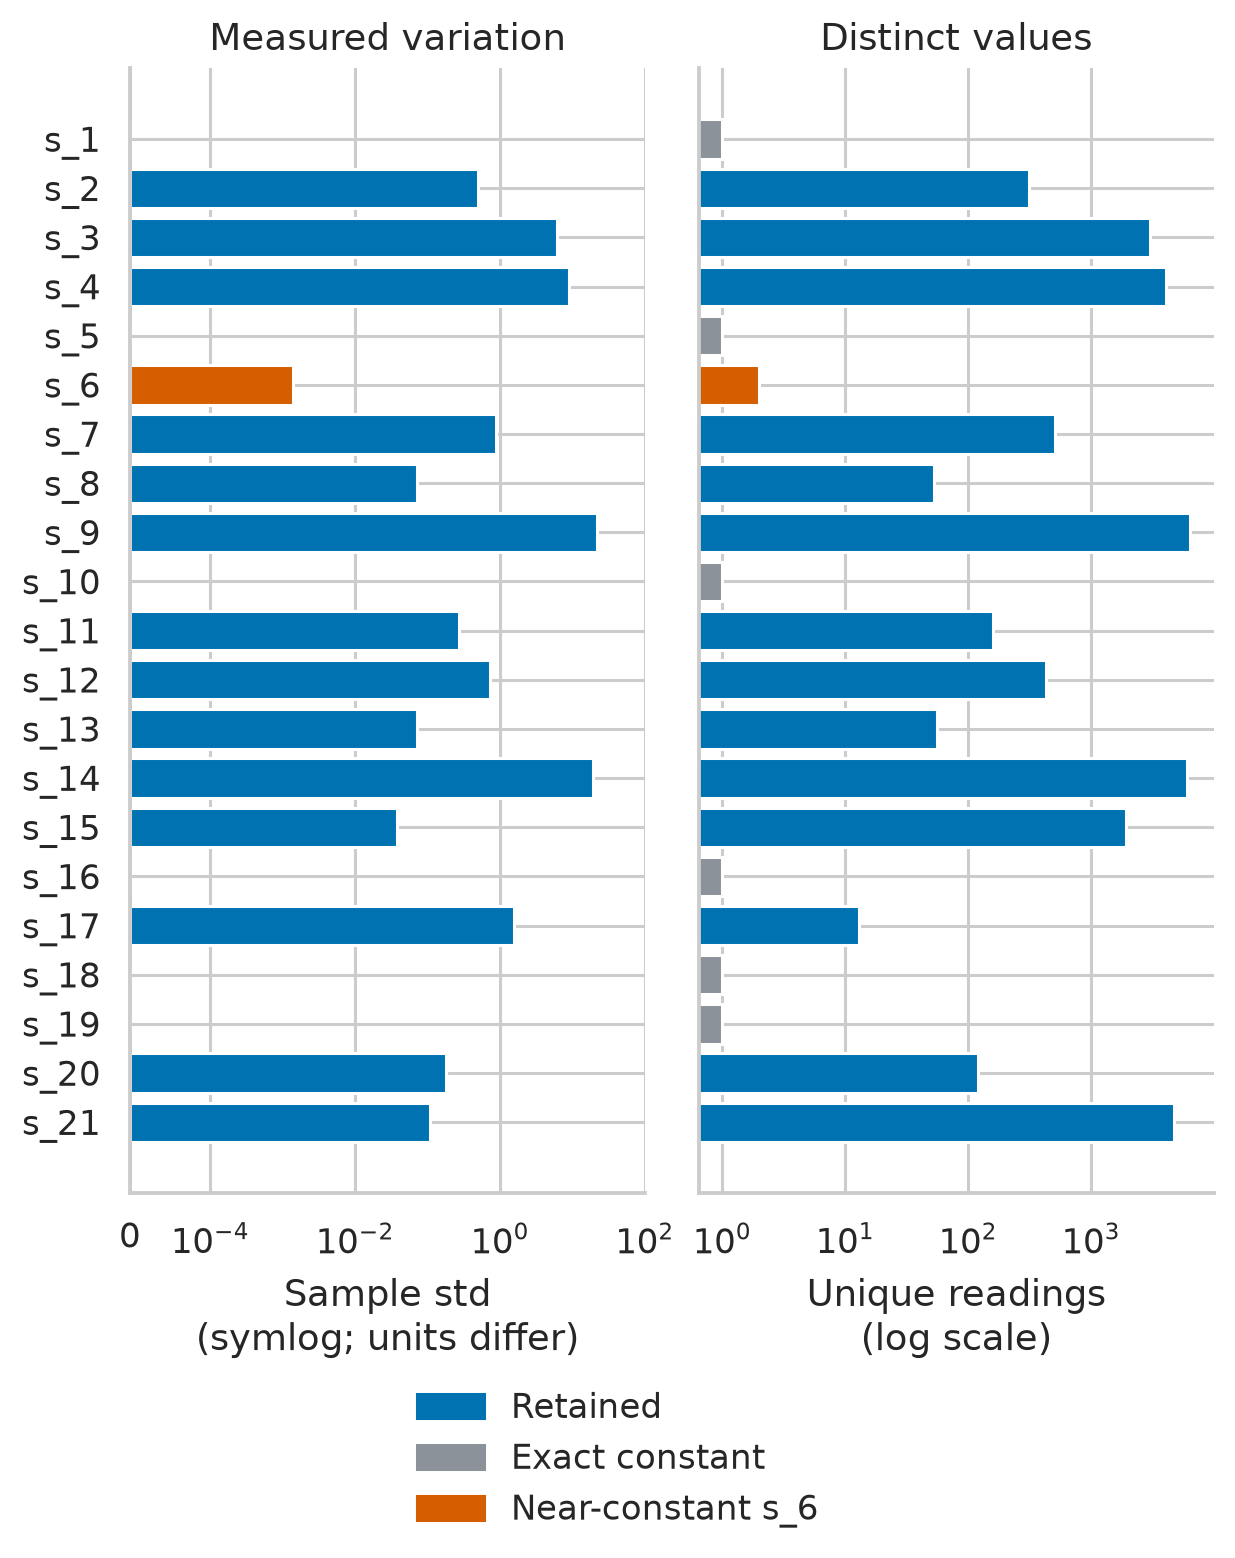
\includegraphics[width=\columnwidth]{../figures/eda_sensor_variation.png}
  \caption{Sensor variation and distinct-value counts. Exact constants are
  shown at zero standard deviation; sensor units differ, so bar lengths
  in the left panel are not directly comparable measures of usefulness.}
  \label{fig:eda-sensors}
\end{figure}

\subsection{Degradation trends and the target cap}
For training engine $i$, let $T_i$ be its final recorded cycle. The uncapped
target at cycle $t$ is $r_{i,t}=T_i-t$, calculated from the complete history.
Figure~\ref{fig:eda-trends} aligns five engines to failure. Engines
9, 44, 65, 76 and 100 are sampled without replacement with seed 42. Faint
curves are raw readings; solid curves use 11-cycle trailing means computed
within each engine, with shorter windows at the start, solely for display.
Several selected sensors show clearer directional changes near failure
than earlier in life, with differing engine baselines and substantial noise.

\begin{figure*}[t]
  \centering
  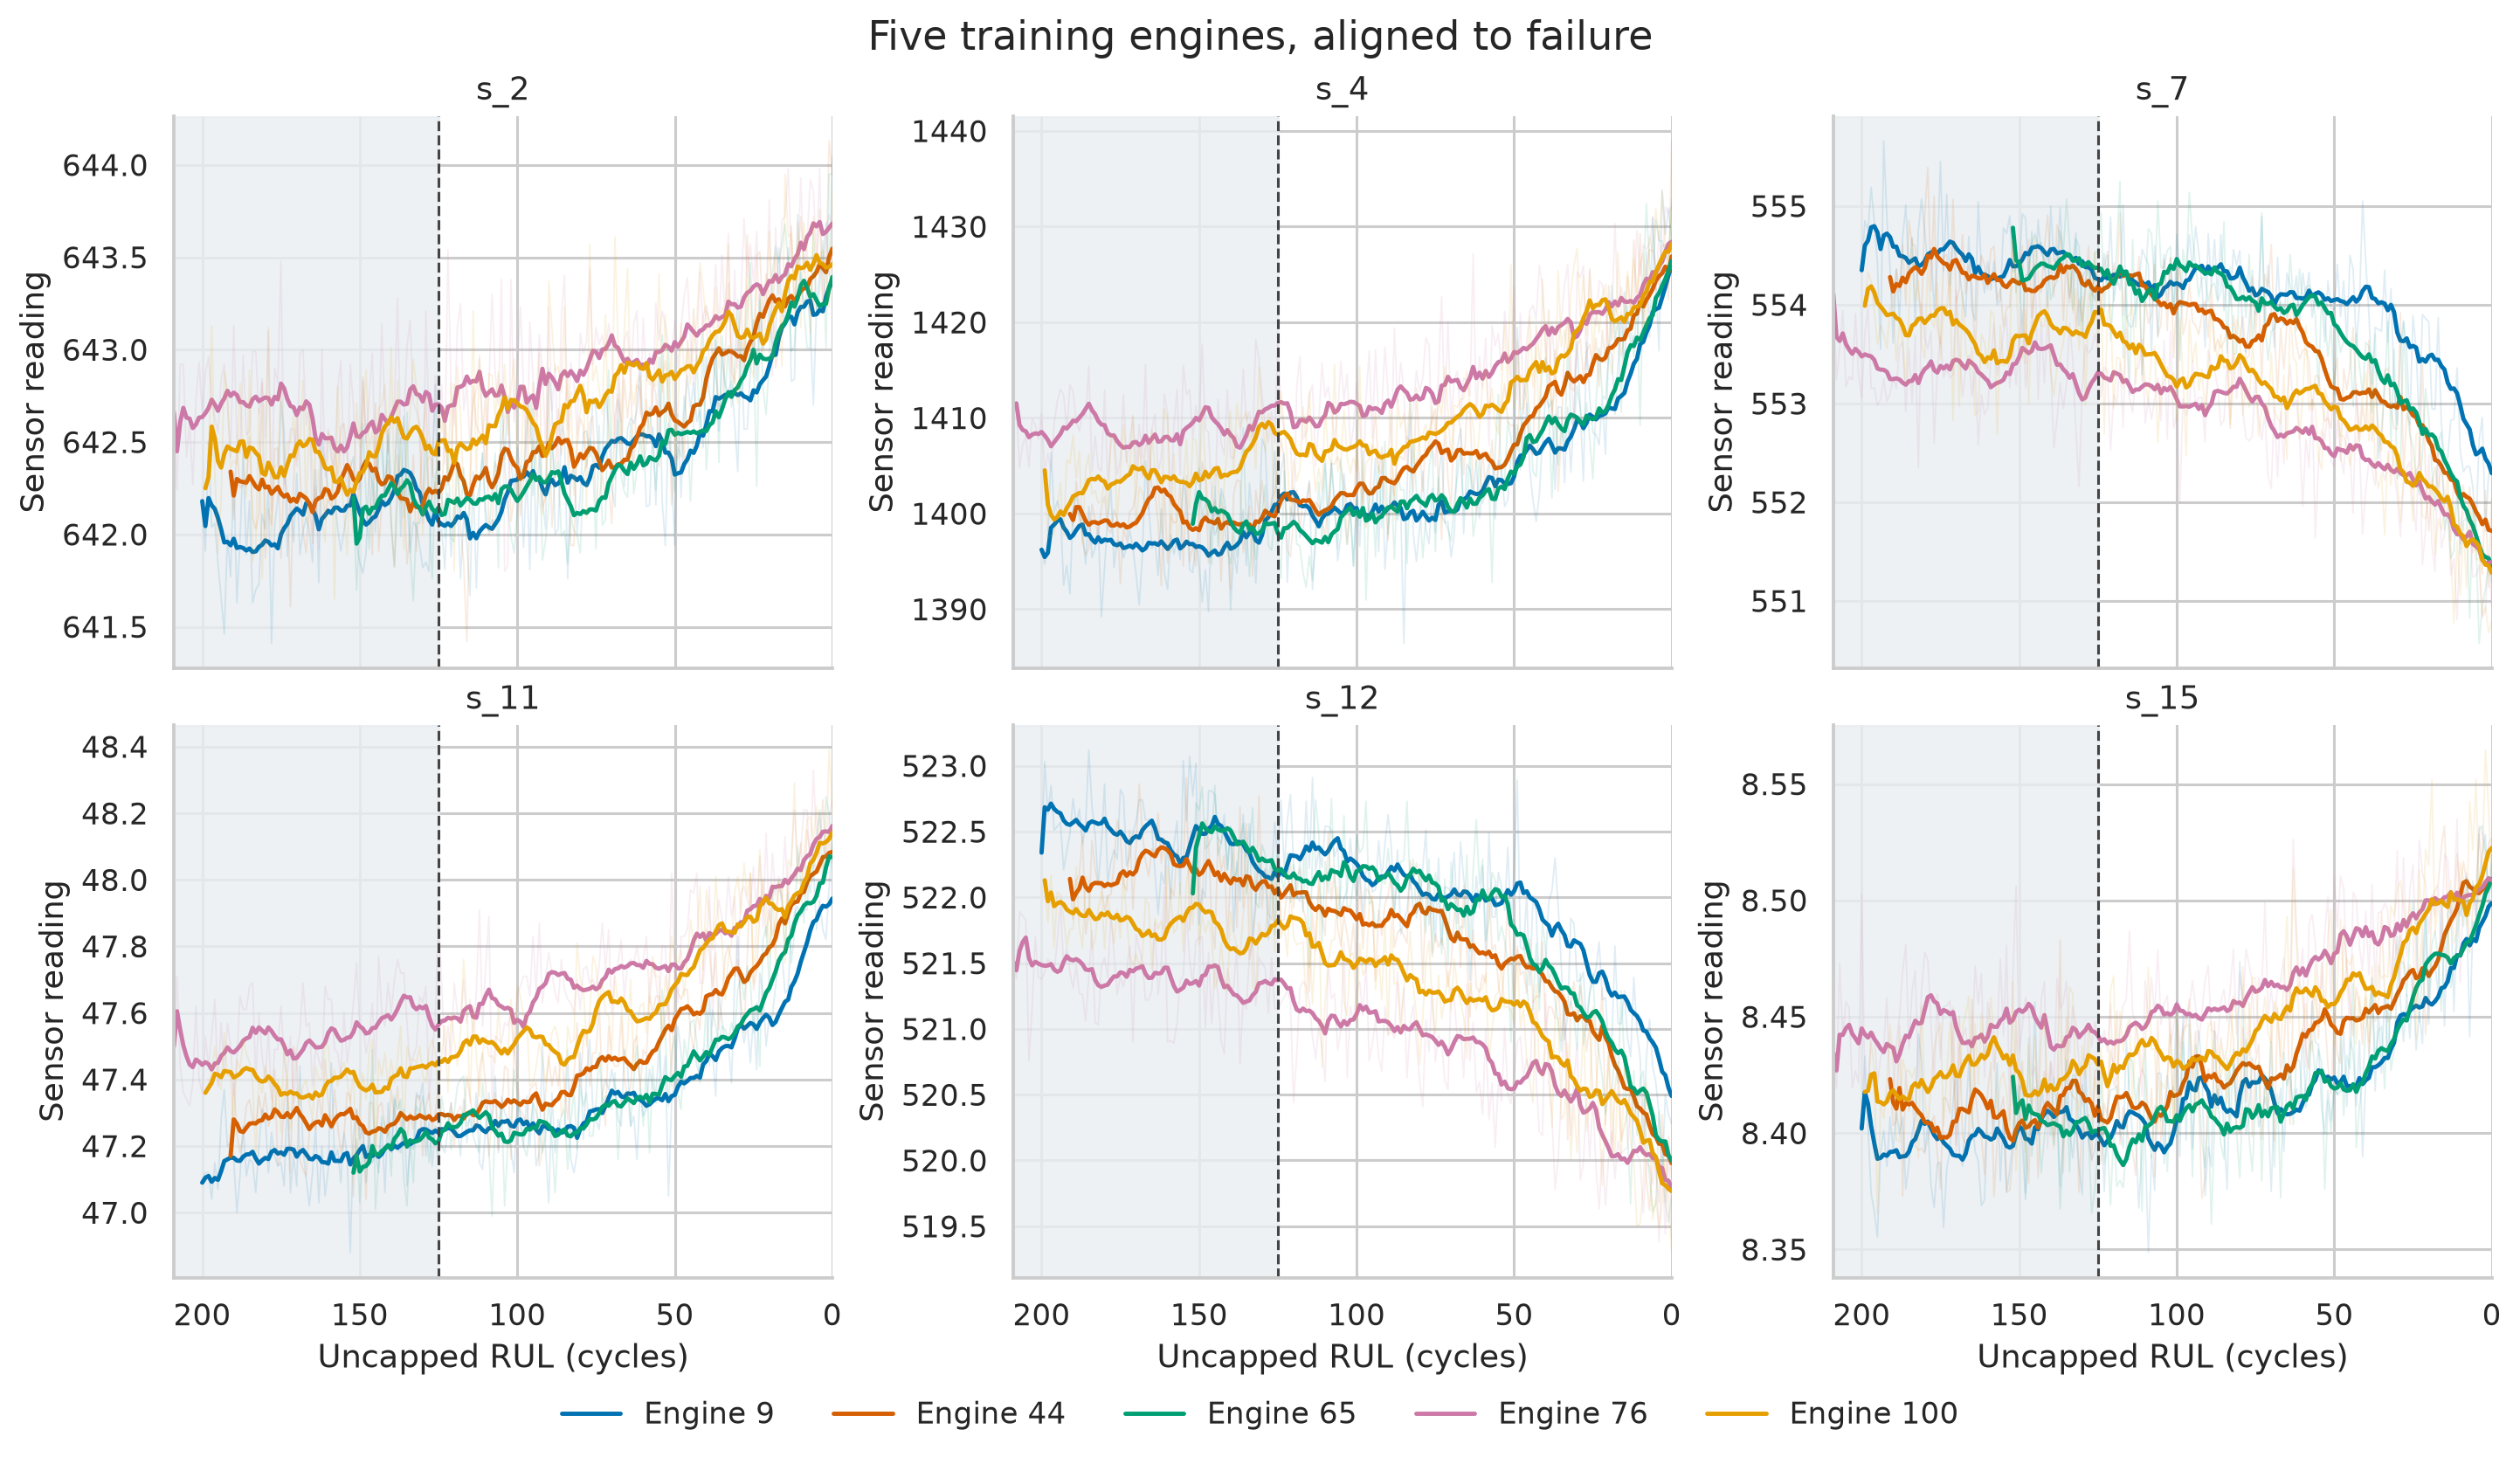
\includegraphics[width=\textwidth]{../figures/eda_sensor_trends.png}
  \caption{Six representative retained sensors from five training engines,
  aligned on uncapped RUL. Failure is at the right. The shaded area has
  RUL above 125; the dashed line marks the team's target cap.}
  \label{fig:eda-trends}
\end{figure*}

We adopt the training target $y_{i,t}=\min(125,r_{i,t})$. Liu, Wang and
Yu~\cite{liu2021rul}, Section 4.2, use an upper target limit of 125 on C-MAPSS
because early sensor evolution carries weak degradation information.
Our plots support this motivation but do not prove that early RUL is
unlearnable or that 125 is optimal. The cap changes 8,031 training labels
(38.93\%). A cap of 100 creates a longer plateau and removes more early-life
target resolution; no cap preserves exact targets but requires distinguishing
more early-life states. The modeling stage compares capped and uncapped
targets with engine-grouped cross-validation. True test RUL remains uncapped.

\subsection{Correlation and limitations}
Figure~\ref{fig:eda-correlation} reports Pearson correlations of the 14
retained sensors and both uncapped and 125-capped training RUL. Several sensors share substantial
variation. We do not remove a sensor solely for correlating with another;
its model-specific contribution requires subsequent evaluation. These are
pooled, row-weighted descriptive associations: adjacent cycles are dependent
and between-engine differences contribute. They do not demonstrate causation
or independent-sample significance, and weak linear association does not
exclude nonlinear or temporal information.

\begin{figure*}[t]
  \centering
  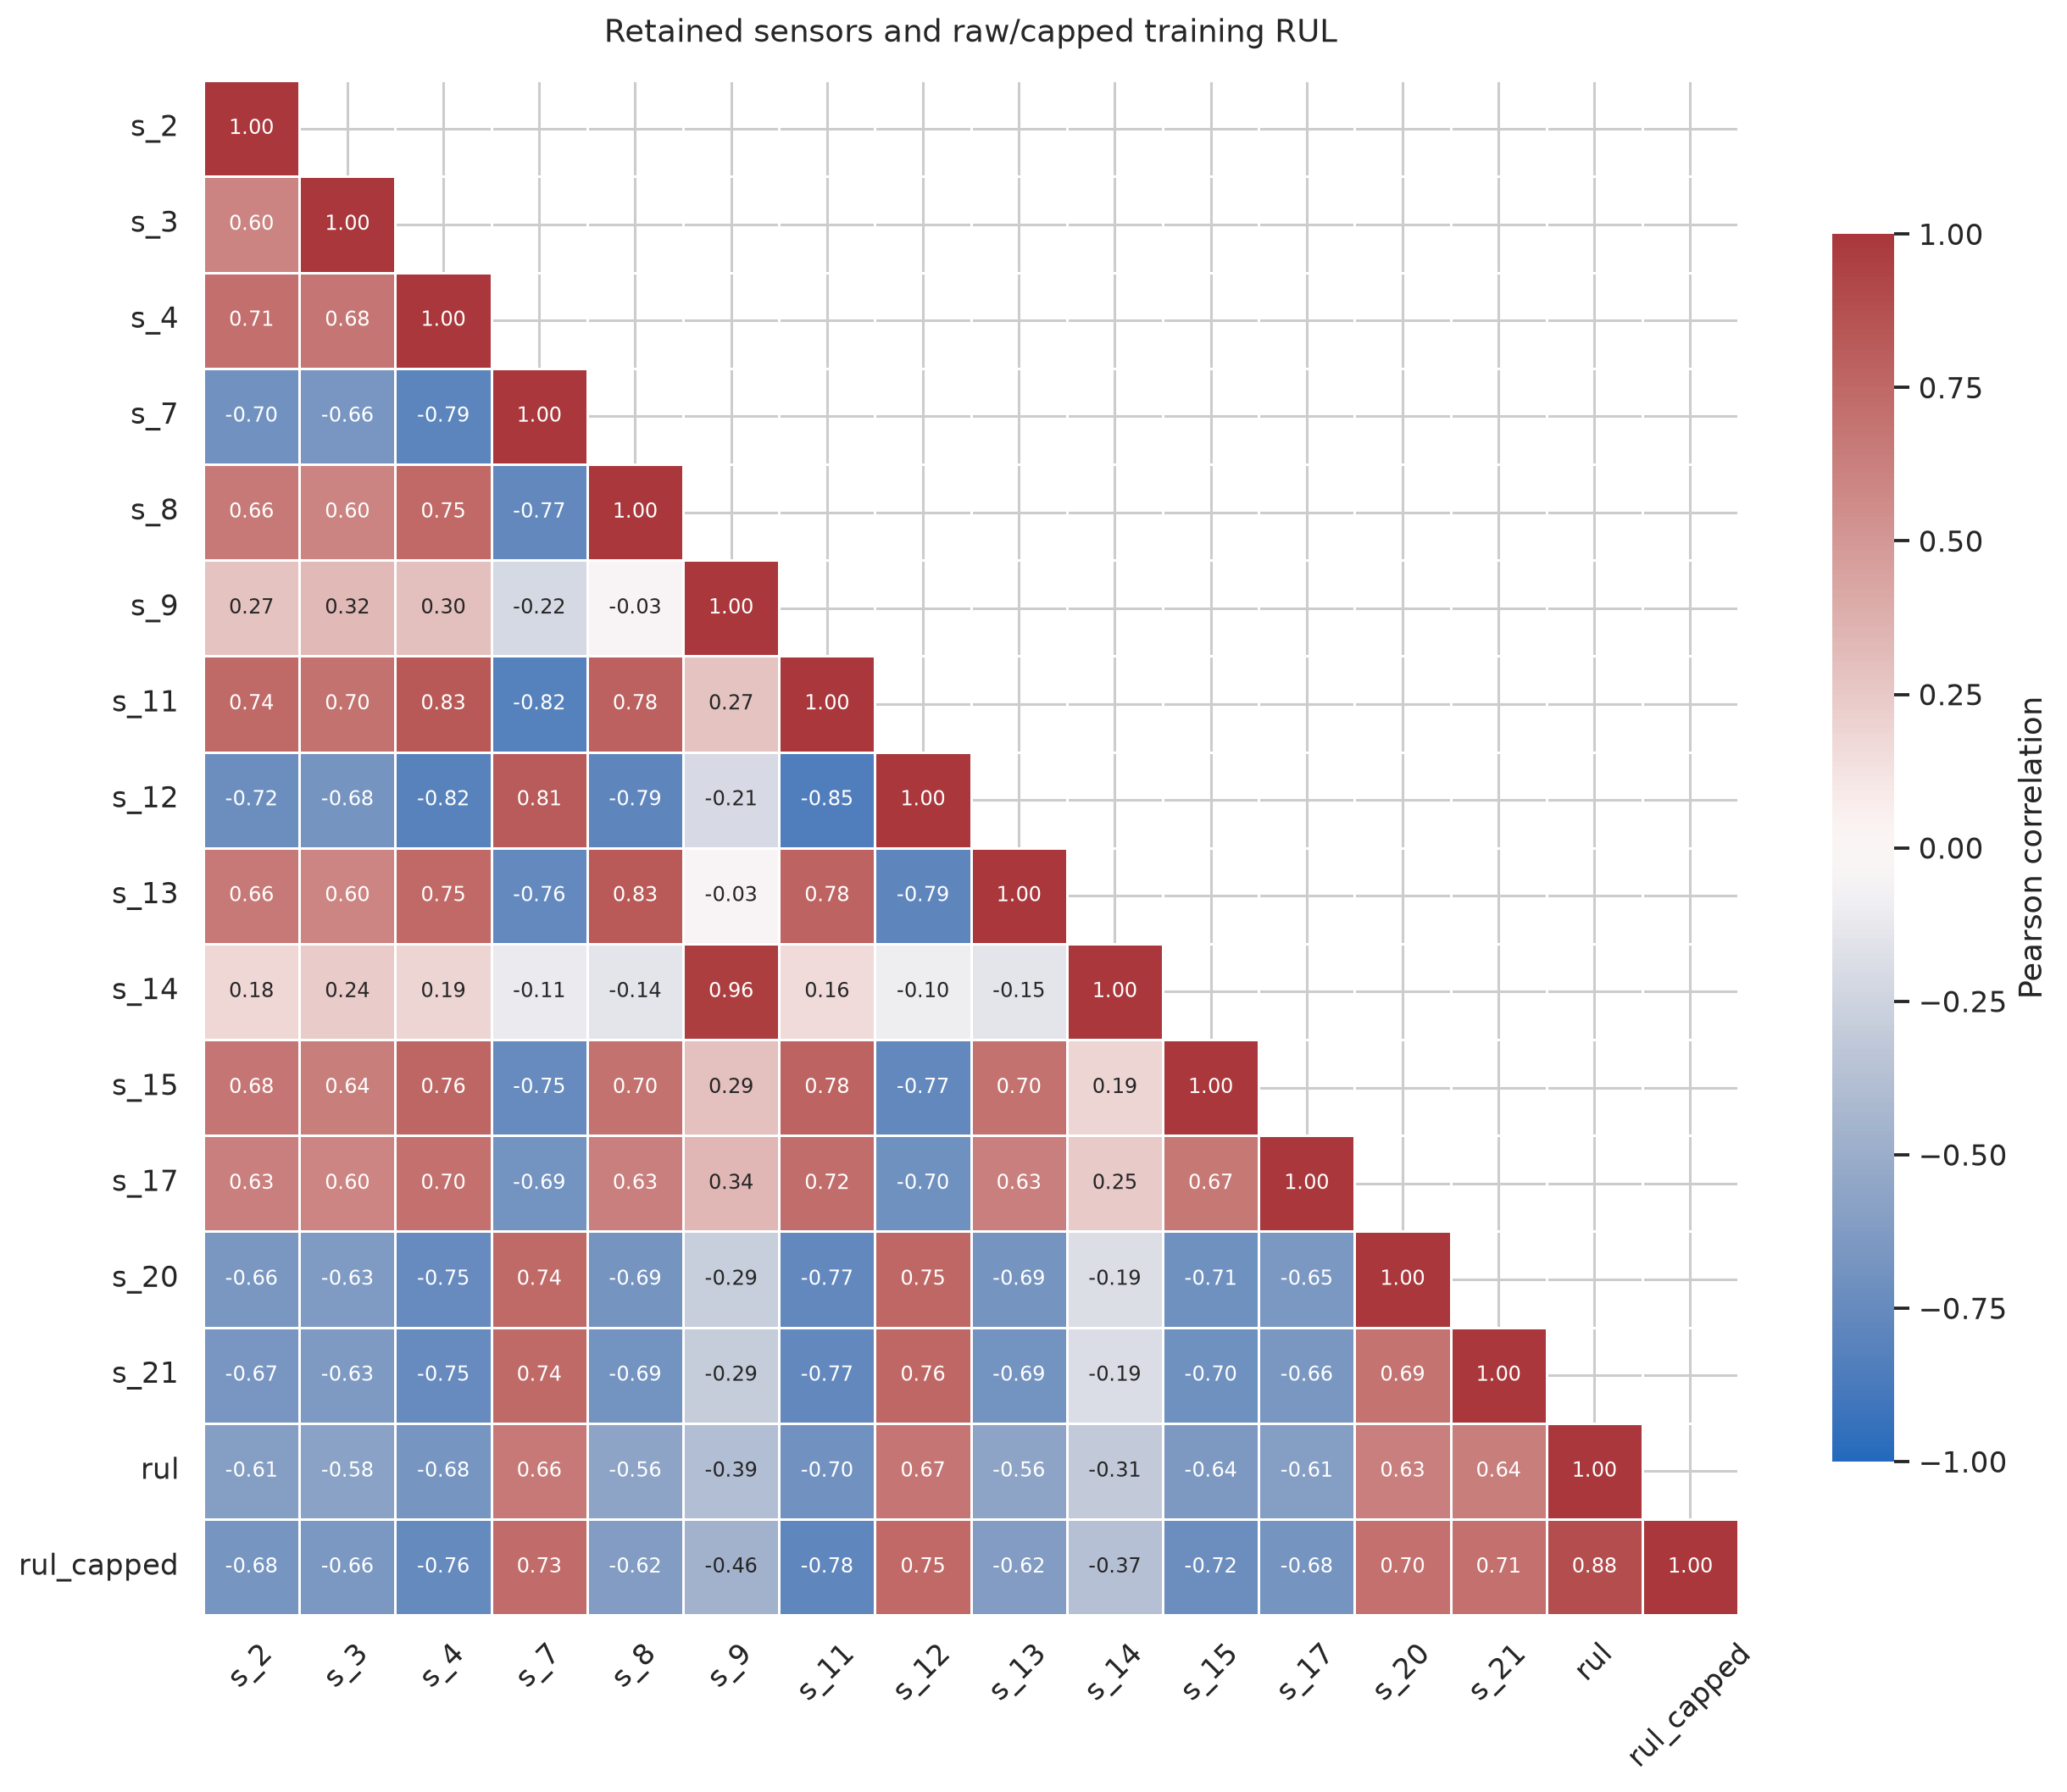
\includegraphics[width=0.85\textwidth]{../figures/eda_correlations.png}
  \caption{Pearson correlations of retained sensors with each other and
  uncapped and 125-capped training RUL. Constants are excluded because their correlations
  are undefined.}
  \label{fig:eda-correlation}
\end{figure*}

This analysis is specific to FD001 and simulated run-to-failure histories.
Sensor selection should be revisited for other operating conditions.
Any learned scaler or feature transformation used in cross-validation must
be fit within its training fold. The notebook retains its outputs and exports
the evidence tables to \texttt{results/eda\_*.csv} for reproducibility.


\subsection{Final descriptive test diagnostics}
After all preceding training decisions, we plot each test engine's last observed
cycle and the distribution of its supplied true RUL (Fig.~\ref{fig:eda-test}).
These are descriptive only; no earlier choice was revisited. Last observed cycle
is a truncation point, not failure or physical engine age. Labels remain uncapped.
No tuning, sensor selection or model evaluation uses these plots.

\begin{figure*}[t]
  \centering
  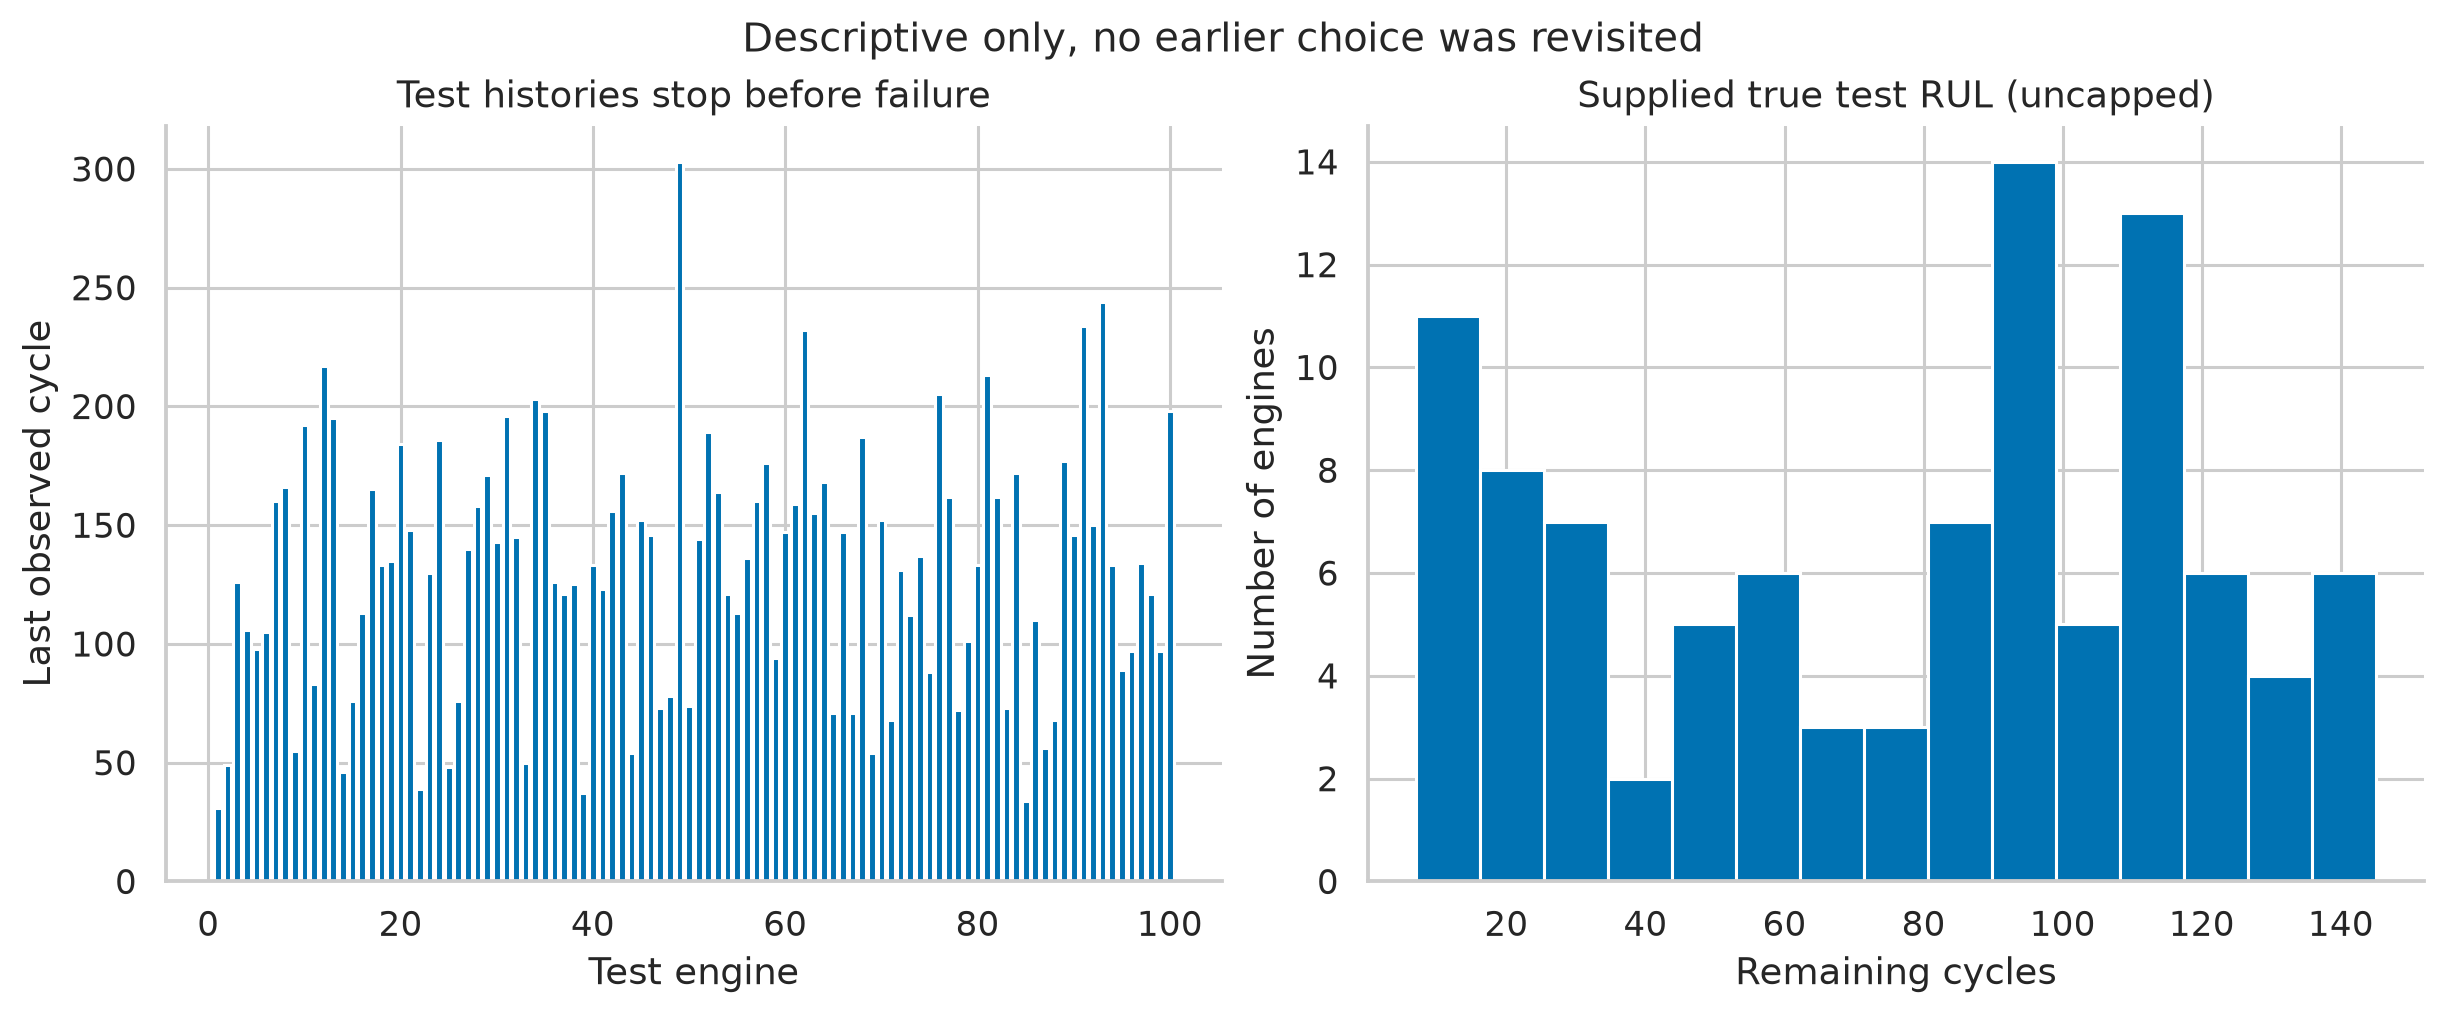
\includegraphics[width=\textwidth]{../figures/eda_test_diagnostics.png}
  \caption{Final test diagnostics: last observed cycle per engine and true RUL
  distribution. Descriptive only, no earlier choice was revisited.}
  \label{fig:eda-test}
\end{figure*}
